\documentclass{article}

\usepackage{amsmath,hyperref}

\newcommand{\Mp}{\ensuremath{{M_{+}}}}
\newcommand{\barMp}{\ensuremath{\overline{\Mp}}}
\newcommand{\Dt}{\ensuremath{\Delta t}}
\newcommand{\tM}[1]{\ensuremath{\tilde{M}(#1)}}
\newcommand{\tMt}{\tM{\tau}}
\newcommand{\tMB}{\ensuremath{{\tilde{M}_B}}}
\newcommand{\tE}[1]{\ensuremath{{\tilde{E}(#1)}}}
\newcommand{\tEt}{\tE{\tau}}

\author{Carl~A.~B.~Pearson}

\usepackage{Sweave}
\begin{document}
\input{synthetic-donations-concordance}
\title{A TEMPLATE}

%\institute{Emerging Pathogens Institute, University of Florida}
\titlepage

\section{A SIMPLE LIST OF POINTS}
\begin{itemize}
\item point one,
\item two,
\item see
\end{itemize}

\section{INSERTING AN R-GENERATED FIGURE}
\begin{figure}
\begin{center}
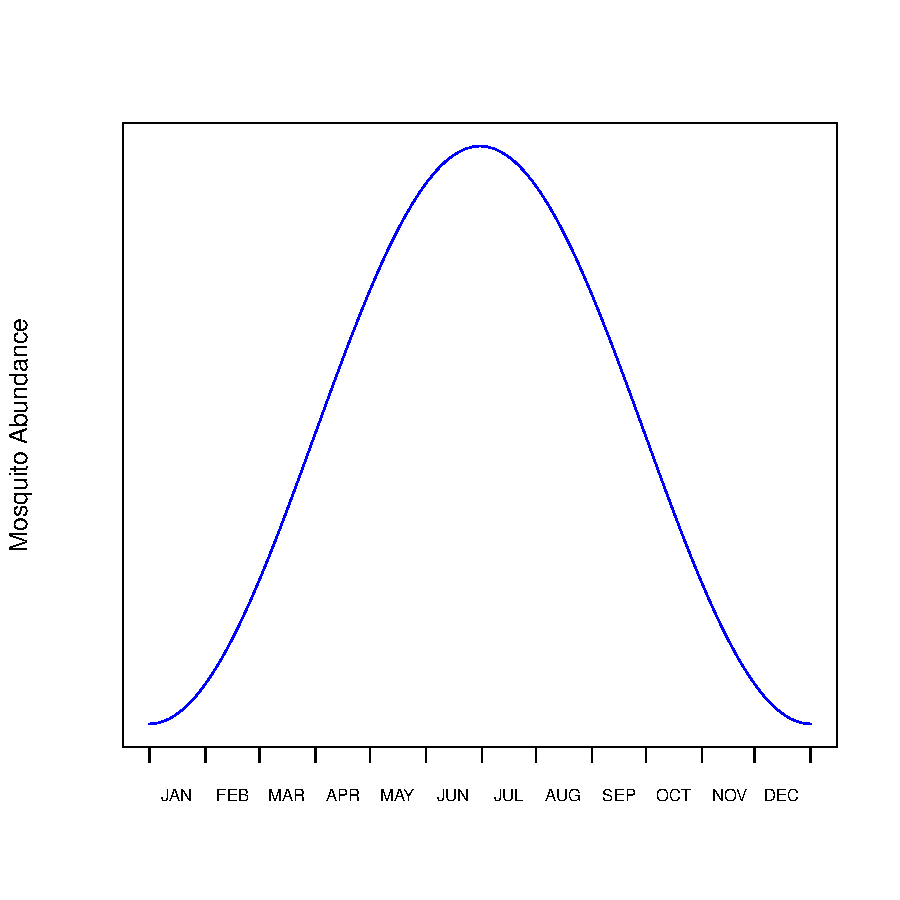
\includegraphics{synthetic-donations-plotfig1}
\end{center}
\end{figure}
% notes-notes-notes

\section{INSERT ANOTHER PDF}
\begin{figure}
\begin{center}
\includegraphics[width=0.9\textwidth]{insert.pdf}
\caption{Bicout et al. J. Med. Entomol. 43(5): 936-946 (2006)}
\end{center}
\end{figure}
% this is a not uncommon measurement of a seasonally varying vector population.

\section{SHOW SOME MATH}
$$
M(t) = C\sin(\omega t+\theta)
$$

\section{SEVERAL EQUATIONS}
\begin{align*}
E(t) &= \begin{cases}
        \dfrac{\Mp}{\Dt} & t \in \Dt \\
        0 & \textrm{otherwise}
        \end{cases}\tag{Step} \\
E(\rho, t) &= \begin{cases}
        \dfrac{2\Mp}{\Dt(2-\rho)} & t \in \Dt(1-\rho) \\
        \dfrac{2\Mp}{\Dt(2-\rho)\rho}\left(1-\dfrac{2|t|}{\Dt}\right) & t \in \rho\Dt \\
        0 & \textrm{otherwise}
        \end{cases}\tag{Modified Step} \\
E(t) &= \dfrac{2\Mp}{\Dt}\sqrt{\dfrac{2}{\pi}}e^{-\dfrac{8t^2}{\Dt^2}}\tag{Approximate $\delta$}
\end{align*}

% DEFINE LOTS OF R...

% THEN USE IT SEVERAL TIMES
\section{THINGS}
\subsection{Modified Step (Trapezoid)}
\begin{figure}
\begin{center}
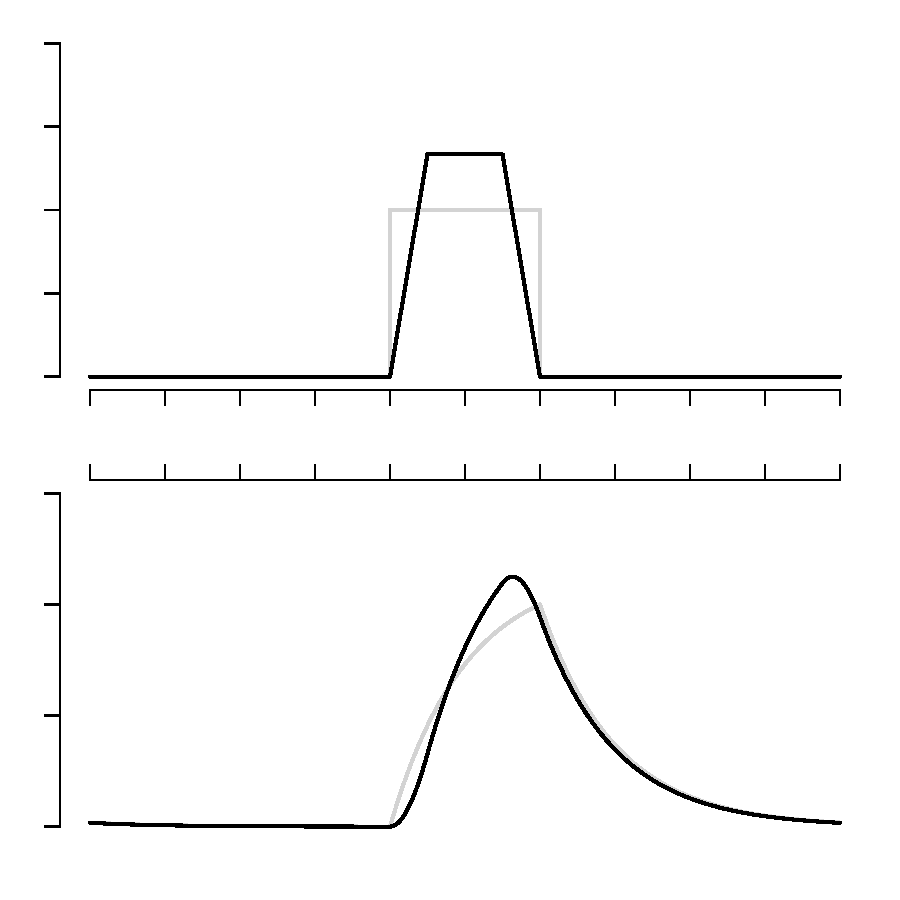
\includegraphics{synthetic-donations-pstrap}
\end{center}
\end{figure}

\subsection{Modified Step (Triangle)}
\begin{figure}
\begin{center}
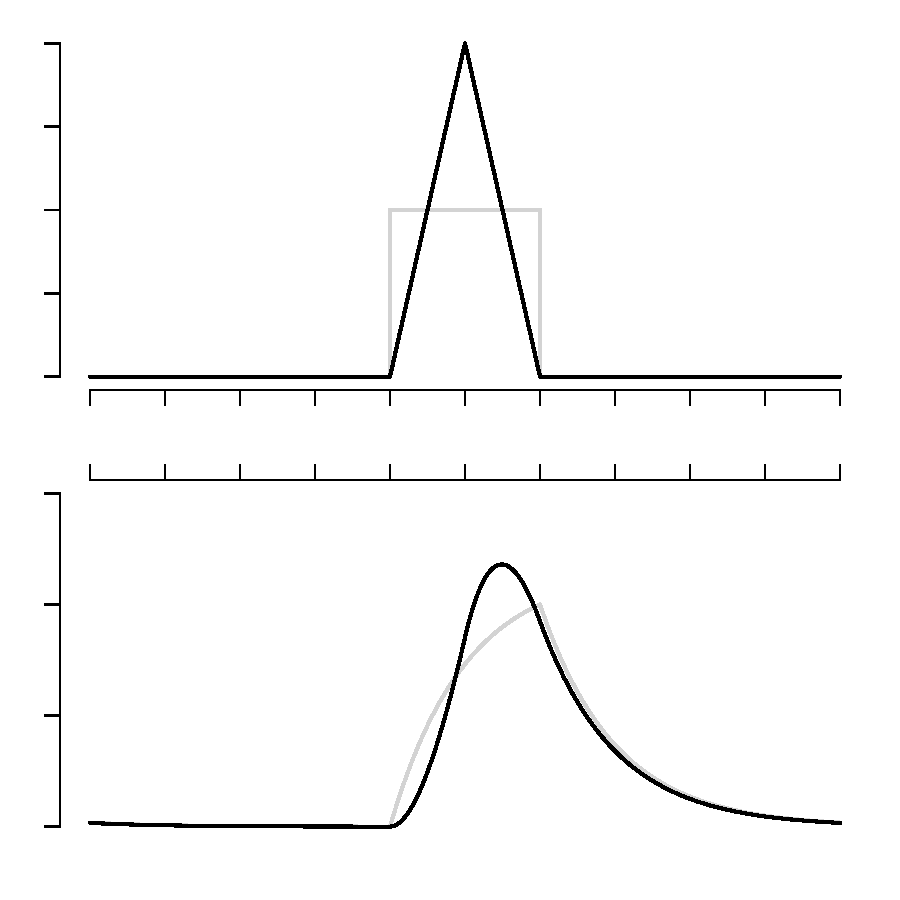
\includegraphics{synthetic-donations-pstri}
\end{center}
\end{figure}

\subsection{Approx. $\delta$}
\begin{figure}
\begin{center}
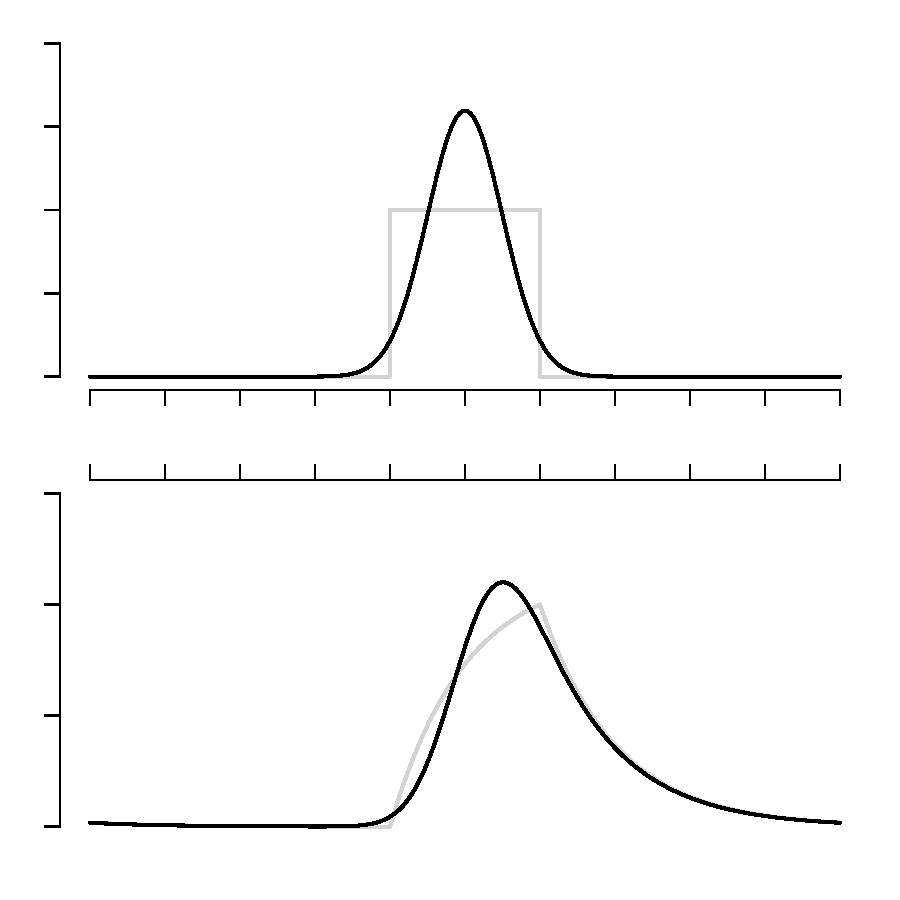
\includegraphics{synthetic-donations-psdel}
\end{center}
\end{figure}

\section{BIBLIOGRAPHY EXAMPLE (CITE ON PREV SLIDE)}
\bibliography{biblio}{}
\bibliographystyle{plain}

\end{document}
